\chapter{Introduction} 
\label{introduction}

Climate change has long been viewed as one of the greatest challenges of the modern era, with governments around the world implementing policies designed to encourage heavy industries and the electrical grid to reduce greenhouse gas emissions. Nuclear energy is anticipated to play a major role in this new low-carbon economy, resulting in an expansion of nuclear generating capacity world-wide. Many reactor vendors are proposing that this expansion be conducted with novel Generation IV reactor designs that have advantages over \acrfull{lwrs} and \acrfull{pthwrs}; some of these advantages include low pressure operation, the use of advanced fuels such as \acrfull{triso} fuel, and high thermal efficiencies \cite{gen_iv_2022_annual_report}. A sample of these technologies include the \acrfull{msr} and \acrfull{htgr}. This next generation nuclear fleet may also adopt \acrfull{smrs} due to their various advantages when compared to conventional facilities, which include a reduced physical footprint, smaller core radionuclide inventories, reduced reactor powers, and decreased plant costs \cite{iaea_2021_fast_reactors, nea_2021_smr_opportunities_challenges}. These new reactor technologies pose many challenges when compared to existing reactors, where the most prominent challenge is a lack of reactor operating experience \cite{iaea_2022_lessons_learned}. Advances in high-performance computing have allowed modelling and simulation to augment the limited existing operational experience and guide further experiments, motivating the development of high-fidelity multiphysics methods for the design and analysis of nuclear systems. 

The main motivation behind the development of new codes is the design of advanced reactors; however, the analysis of these new reactors for the purposes of safety and determining their environmental impact is also of importance. The aim of this work is to develop a series of high-fidelity methods useful for health physics and environmental impact applications, filling a gap that exists for safety analysis. This chapter aims to provide context to the need for these methods, starting with a discussion of health physics concerns posed by the development of advanced reactors. This is followed by a description of the \acrfull{moose} and \texttt{Caribou}, a health physics and environmental impact code built on \acrshort{moose} which this work contributes to.

\section{Health Physics Concerns in Advanced Reactors}
\label{introduction:hp_advanced}

Nuclear safety analysis and environmental impact assessments verify that a nuclear plant meets the high-level safety goals of the regulator (i.e. a maximum allowed radiation dose) prior to construction or modification \cite{regdoc_2_4_1, regdoc_2_5_2}; a necessary step along the path to deployment which is required by national regulatory bodies such as the \acrfull{cnsc}. The technological benefits of Generation IV reactors and \acrshort{smrs} have resulted in several licensing challenges with regards to environmental impact and nuclear safety. \acrshort{triso} fuels are layered such that the fuel itself acts as a series of containment boundaries \cite{triso_ref_piro}, and so \acrshort{htgr} reactor vendors are proposing that these designs do not need separate containment structures and exclusion zones \cite{iaea_2022_lessons_learned}. Removing the containment structure and exclusion zone places additional scrutiny on existing reactor components and system boundaries, motivating the use of analysis methods which reduce uncertainty in high-level safety metrics. \acrshort{msr}s use a liquid fuel salt as opposed to traditional solid fuel assemblies. The piping required to move fuel from the reactor vessel to a primary heat exchangers results in long radiation streaming paths, complicating the design of shielding and presenting another radiation hazard. Many of these novel reactors operate with a different neutron spectrum and a higher fuel enrichment, resulting in ex-core\footnote{Recent advances in reactor multi-physics methods have addressed in-core nuclide inventories for Generation IV reactors, and so the focus of this work is on ex-core radionuclide sources.} radionuclide inventories which differ from the current fleet of \acrshort{lwrs} and \acrshort{pthwrs}. \acrshort{smrs} have higher leakage fractions then conventional power reactors. This couples with smaller containment systems, which may result in an increased formation of mobile effluents along with higher structural material activation rates per unit of reactor power. These transmutation products pose a challenge to analysis methods which use empirical correlations as these simplified methods have largely been derived for \acrshort{lwrs} and \acrshort{pthwrs}.

New computational tools can assist in mitigating the previously discussed health physics concerns inherent to novel reactor technologies. Neutral particle transport and nuclide dispersion are two phenomena that require modelling for safety analyses, environmental impact assessments, operational work planning, and the design of shielding. Simulating the behavior of neutrons and gamma photons emitted by a nuclear reactor into the containment system yields insight into the evolution of radionuclide inventories, while also providing direct radiation fields useful for determining radiation dose rates and the design of the reactor biological shield. The simulation of secondary gamma photon fields generated by the decay of these in-containment radiation source terms also proves to be invaluable for outage work planning and the selection of portable photon shielding used to perform maintenance tasks. Modelling radionuclide dispersion becomes necessary when evaluating the environmental impact of highly mobile radionuclide effluents (e.g., $\mathrm{^{3}H}$, $\mathrm{^{14}C}$, and $\mathrm{^{41}Ar}$) formed during normal operations, and the dose consequences caused by the controlled release of core materials during an accident sequence. In the latter case nuclides of importance to accident analysis such as $\mathrm{^{137}Cs}$ \cite{regdoc_2_5_2} have decay chains which include isomeric transitions, resulting in photon emissions in the form of gamma radiation. This necessitates the use of photon transport to calculate the external dose from the emission, and dispersion methods to compute the evolution of the spatial distribution of nuclides over time. Finally, high-fidelity methods can reduce uncertainties in radiation dose predictions to support the case for removing containment structures and shrinking exclusion zones. 

\section{Multi-Physics Simulations for Health Physics Applications}
\label{introduction:ms}

Previous methods for evaluating the environmental impact of nuclear facilities were largely confined to low-fidelity atmospheric and aqueous dispersion methods using experimentally determined dispersion coefficients, coupled with simplified analytical solutions for radiation fields produced by the plume for computing external radiation doses \cite{nf_rdd_trials_i,nf_rdd_trials_ii,n_288_1_20,n_288_2_19}. The concentration of highly mobile radionuclide effluents are computed using simplified neutron flux models and transfer functions to account for the movement of radionuclides between different control volumes, such as the containment building to the atmosphere \cite{ar41_triga_1,n_288_1_20}. Recent developments in computational methods and high performance computing allow for the use of multi-scale, multiphysics methods to enable the modelling of physical phenomena which was previously ignored to err on the side of conservatism. This reduces the uncertainty in calculations used to support the licensing of facilities and aids in guiding experimental work required for site and reactor characterisation.

\begin{figure}[H]
    \centering
    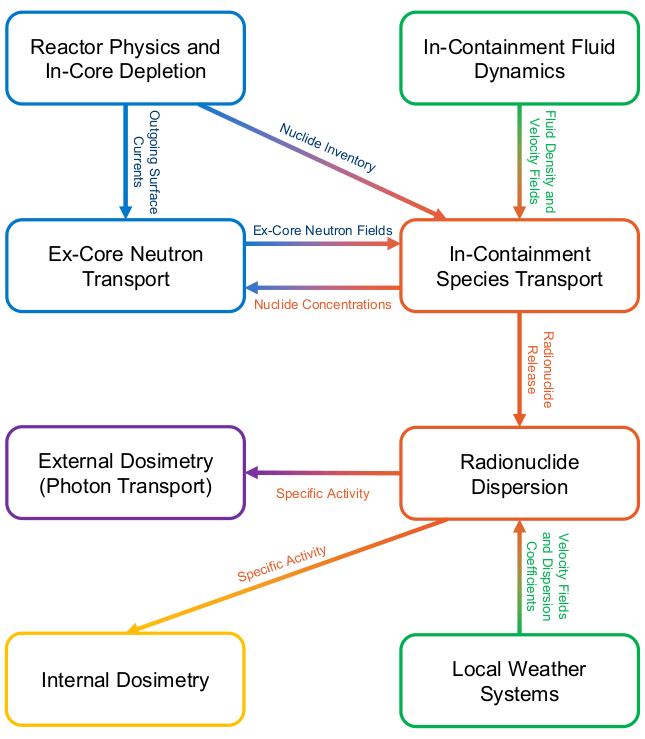
\includegraphics[width=0.65\textwidth]{images/introduction/release_multiphysics.png}
    \caption{Multiphysics phenomena in an airborne release of radioactive material.}
    \label{fig:introduction:ms:physics}
\end{figure}

The formation of nuclides in ex-core radiation fields, the transport of nuclides, and the resulting dosimetry concerns span many different physics and cover several different length scales. As an example, consider the various phenomena involved in an airborne radioactive release from a reactor containment building (Figure~\ref{fig:introduction:ms:physics}). Neutron transport within the containment building takes place over length scales of centimeters to metres and times scales of nanoseconds to microseconds. The formation and transport of effluents within containment is governed by the resulting neutron fields and airflow within containment, with length scales from metres to tens of metres and time scales on the order of seconds to minutes. The atmospheric dispersion of releases takes place over length scales of hundreds of metres to kilometres and time scales of hours to days. This is dependant on local weather patterns, the complexities of the terrain surrounding the nuclear facility, and the local built environment. Finally, external photon dosimetry is concerned with length scales that range from metres to hundreds of metres (depending on the activity of the release) and time scales on the order of nanoseconds to milliseconds. It is clear that a multiphysics approach which considers these differences in length and time scales are required for modern computational methods used to evaluate the environmental impact of nuclear facilities.

\subsection{The Multiphysics Object Oriented Simulation Environment}
\label{introduction:ms:moose}

The need to move towards a multiphysics and multi-scale approach for analysis of many nuclear systems resulted in the development of the \acrshort{moose}, an open-source simulation framework designed to take advantage of recent advances in massively parallel computing to solve larges systems of partial differential equations \cite{moose_0,moose_1,moose_2}. \acrshort{moose} was initially developed at \acrfull{inl} with the main aim of abstracting the more complicated tasks that are required to develop a new analysis code, such as the machinery of numerical discretization and the sparse linear algebra required to solve the resulting system of nonlinear equations. To enable this functionality, \acrshort{moose} wraps the \acrfull{petsc} \cite{petsc_manual} for state of the art sparse matrix solution algorithms and libMesh \cite{libmesh} for finite element and finite volume discretization schemes. \acrshort{moose} provides many other features which make it more suitable for multiphysics calculations than competing frameworks. These include \acrfull{ad} \cite{moose_ad}, automatic documentation and quality assurance to NQA-1 \cite{moose_civet}, in memory coupling between different \acrshort{moose} applications \cite{moose_coupling}, and a plethora of common physics modules \cite{moose_ns_summary,moose_th,moose_reactor}. Of particular importance to this work is the \texttt{NavierStokes} module \cite{moose_ns_summary,moose_ns_crab}, which includes capabilities used by the coarse-mesh thermal-hydraulics code \texttt{Pronghorn} developed at \acrshort{inl}.

There are many \acrshort{moose}-based applications (both open-source and export controlled) which have been developed for modelling nuclear reactors and other nuclear systems. These include export controlled codes such as \texttt{Griffin} \cite{griffin_sdp} for in-core radiation transport and nuclide depletion, \texttt{Pronghorn} \cite{moose_ns_crab} for coarse-mesh computational fluid dynamics, and \texttt{Yellowjacket} \cite{yellowjacket} for corrosion and fuel chemistry. Open-source applications include \texttt{Moltres} \cite{moltres} for the simulation of coupled \acrshort{msr} neutron diffusion and thermal-hydraulics, and \texttt{Cardinal} \cite{cardinal} for high-fidelity multiphysics simulations using Monte Carlo radiation transport (through \texttt{OpenMC} \cite{openmc}) and spectral elements \acrfull{cfd} (using \texttt{NekRS}). 

While the \acrshort{moose} ecosystem contains many applications with wide ranging capabilities it still lacks a dedicated tool for performing health physics and environmental impact analysis. The reactor physics applications \texttt{Griffin} and \texttt{Cardinal} can be used to fill some of the requirement of a health physics code, namely external dosimetry and ex-core neutron transport. However, there are several disadvantages to taking this approach. The use of \texttt{Griffin} would necessitate that any capabilities added to facilitate health physics analysis be placed under export control. The use of \texttt{Cardinal} for long length scale radiation transport problems such as  ex-core activation and shielding analysis is largely impractical due to the lack of deterministic variance reduction techniques, yielding increasingly large uncertainties in tallies as one moves away from the reactor core or radionuclide sources. The \texttt{NavierStokes} module can solve for radionuclide distributions within fluids over short length scales, such as in fission reactor cores and containment systems. However, there is no capability built in \acrshort{moose} to integrate either aqueous or atmospheric dispersion of radioactive releases with meso scale weather models over length scales of kilometers. To address this gap in capabilities a new multiphysics health physics and environmental impact code named \texttt{Caribou} is under development at Ontario Tech\footnote{The development of \texttt{Caribou} if being performed independently without any collaborations with \acrshort{inl}.}. The work performed in this thesis contributes to this new code, adding a near-field radiation transport and trace species transport solver to \texttt{Caribou}. Its relationship to, and a description of \texttt{Caribou} are described in the following section.

\subsection{Caribou}
\label{introduction:ms:caribou}

As a response to the health physics and environmental challenges posed by Generation IV reactors and \acrshort{smrs}, \texttt{Caribou} is designed to enable predictive modelling of static and transient radiological events within a multiphysics and multi-scale framework. \texttt{Caribou} has two main objectives: to reduce uncertainties across various length scales, and to provide high quality reference data to more accurately predict radiological consequences after a nuclear accident. As shown in Figure~\ref{fig:introduction:ms:caribou:caribou}, \texttt{Caribou} will contain capabilities for neutral particle transport, radionuclide species transport, and \acrshort{cfd}. The methods required to simulate species transport change depending on the fluid the radionuclides are suspended in and the length scale under consideration. \texttt{Caribou} handles this difficulty by first differentiating species transport by length scale, where near-field transport occurs at lengths of tens to hundreds of meters and far-field transport occurs at distances greater than one kilometer. The far-field species transport is then further separated into atmospheric dispersion and aqueous dispersion owing to the differences in underlying fluid and weather modelling required to simulate species transport in those cases. The development of the far-field dispersion capabilities along with coupling these capabilities to meso scale weather models are the subjects of additional research efforts at Ontario Tech, while this work focuses on near-field radiation transport and trace species transport.

\begin{figure}[H]
    \centering
    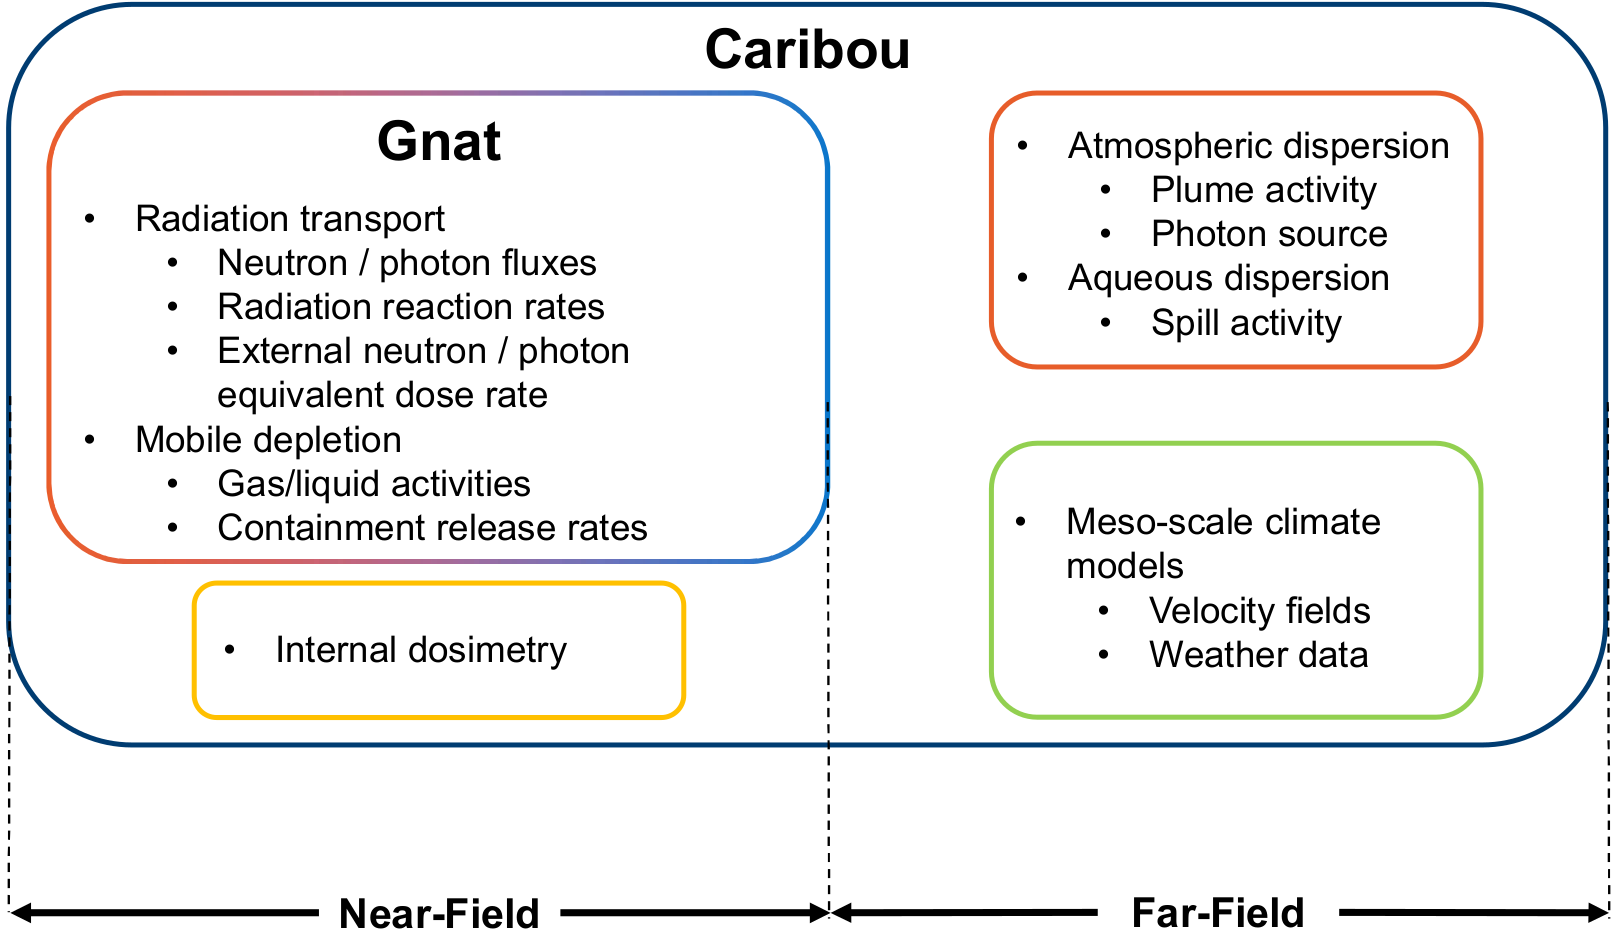
\includegraphics[width=1.0\textwidth]{images/introduction/caribou.png}
    \caption{Current and planned capabilities of \texttt{Caribou}.}
    \label{fig:introduction:ms:caribou:caribou}
\end{figure}

Near-field capabilities, such as radiation transport and the transport of radioactive trace species, are valuable capabilities for \texttt{Caribou} to have. Neutron transport within containment systems allow analysts to compute ex-core nuclide source terms, which may be released during a nuclear accident. Coupling neutron transport with trace species transport allows for the computation of gaseous / liquid source terms, such as $\mathrm{^{16}N}$ or $\mathrm{^{41}Ar}$ activities and predicting their behaviour. These potentially novel source terms can be provided to the far-field dispersion models entirely within \texttt{Caribou}, avoiding the need to couple together separate codes. Finally, the far-field dispersion models can propagate nuclide activities to the near-field trace species and gamma photon transport solver, allowing for high-fidelity external dose calculations at length scales of meters. Throughout this work, the transmutation of a fluid in a neutron field is referred to as mobile depletion to emphasize the connection with depletion in reactor cores as both share similar numerical challenges. The main motivation behind this work was to enable direct radiation transport, mobile depletion, and the coupling of both physics together within \texttt{Caribou}. This resulted in a \acrshort{moose} mini-application distributed with \texttt{Caribou} called the \acrfull{gnat}. The objectives, tasks, and deliverables of this work are described in the following chapter.

\section{Thesis Structure}
\label{introduction:ms:structure}

The remainder of this thesis is organized as follows. Chapter~\ref{statement_of_work} presents the objectives of the work and the related research tasks. Chapter~\ref{lit_review} provides a literature review on radiation transport methods, trace species transport methods, and previous approaches used for coupled radiation transport and mobile depletion. Chapter~\ref{solver} provides a description of \acrshort{gnat}, the radiation transport and mobile depletion solver implemented as a part of \texttt{Caribou} through this work. Chapter~\ref{verification} discusses the steps taken to verify the solver and provides verification results. Chapter~\ref{demos} presents a series of demonstration problems which showcase the capabilities of \acrshort{gnat}. The work is concluded in Chapter~\ref{conclusion}, and recommendations for future study are provided in Chapter~\ref{recommendations}.